\begin{table}[ht]
    \centering
    \begin{tabular}{l|lrr}
        \textbf{Developer} & \textbf{Model} & \textbf{\#Param} & \textbf{\$ per M/Tok} \\
        \hline
        OpenAI  & gpt-3.5-turbo     & ${\dagger}$ & 00.50/01.50 \\
        ~       & gpt-4             & ${\dagger}$ & 30.00/60.00 \\
        ~       & gpt-4-turbo       & ${\dagger}$ & 10.00/30.00 \\
        ~       & gpt-4o           & ${\dagger}$ & 05.00/15.00 \\
        ~       & ~                 & ~             & ~     \\
        Google  & gemini-1.0-pro    & ${\dagger}$ & 00.50/01.50 \\
        ~       & gemini-1.5-flash  & ${\dagger}$ & 00.35/01.05 \\
        ~       & gemini-1.5-pro    & ${\dagger}$ & 03.50/10.50 \\
        ~       & ~                 & ~             & ~     \\
        Anthropic & claude-3-opus & ${\dagger}$ & 15.00/75.00 \\
        ~       & claude-3-sonnet & ${\dagger}$ & 03.00/15.00 \\
        ~       & claude-3-haiku & ${\dagger}$ & 00.25/01.25 \\
        ~       & ~                         & ~             & ~      \\
        Meta    & llama3-70b        & 70b       & 03.20/03.20 \\
        ~       & llama3-8b         & 8b        & 01.60/01.60 \\
        ~       & ~                         & ~             & ~      \\
        Mistral & mixtral-8x22b-instruct & 39b/141b  & 03.20/03.20 \\
        ~       & mistral-7b-instruct & 7b     & 01.60/01.60 \\
    \end{tabular}
    \caption{Summary of models evaluated.${\dagger}$ denotes where information has not been publicly disclosed.}
    \label{tab:models}
\end{table}

\section{Results}
\label{section:results}

In this section we discuss the results of the experiments described in the previous section.

\subsection{Result 1: Toponym Resolution}

\begin{figure}
    \centering
    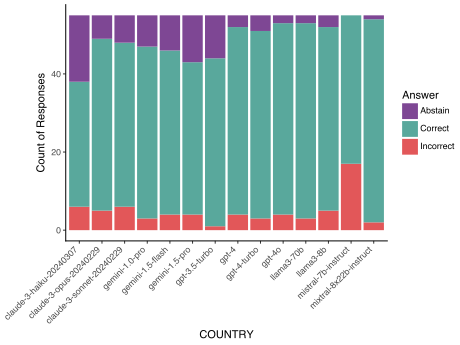
\includegraphics[width=\columnwidth]{figures/toponym_bar_country}
    \caption{Toponym resolution results for base LLMs. Most models resolve most toponyms to Australia. }
    \label{fig:toponym}
\end{figure}

\textbf{Most toponyms are resolved correctly.}
The toponym experiments shown in figure~\ref{fig:toponym} show percentage of responses that were correct, incorrect and abstain from answering. 
Most models are capable of answering toponym resolution questions, with the majority of abstains associated with the less popular or Indigenous place names. 
\texttt{Mistral-7b-instruct} produced excessive tokens when answering questions, contributing to its increased error rate, whereas \texttt{gpt-4} resolved toponyms like `Port Arthur', `Exmouth' and `Roma' to Texas, the United Kingdom and Italy respectively.
These are valid resolutions, but could cause cause correct spatial reasoning to be marked incorrectly, if the model is considering different locations to what the question intended.
To avoid this issue, we ensure than none of the toponyms marked incorrectly in toponym resolution appear together in questions, so that the models should infer the correct resolution given the context of the other toponyms resolved to Australia.



\subsection{Result 2: Directional Relations}
\textbf{Performance degrades when adding 3rd directional relation.}
The results for the $22$ 2-way directional prompts in figure~\ref{fig:direcional-2} varied across the models, with \texttt{claude-3-haiku} unable to answer any question and \texttt{mistral-7b-instruct} again struggling because of token over-generation. 
For comparison, \citeauthor{Qi2023} performed 2-way directional prompting for major cities in Australia and found the responses to be correct in 44 out of 50 cases~\cite{Qi2023}.
The tests for the $20$ 3-way prompts summarized in Figure~\ref{fig:directional-3} show that half of the models tested had a significant increase in error rate over the 2-way directional prompts and the other half abstained from answering all or nearly all of the 3-way directional questions.



\begin{figure*}[ht]
    \centering
    \begin{subfigure}[Model performance on 2-way directional relation prompts. Results indicate better performance by OpenAI models compared to the other models tested.]{
        \includesvg[width=\columnwidth]{figures/directional_bar_2-way}
        \label{fig:direcional-2}
        }
    \end{subfigure}
    \hfill
    \begin{subfigure}[Model performance on 3-way directional relation prompts. A third constraint decreases answer confidence and accuracy. OpenAI models still outperform others, but at a much lower rate of success.]{
        \includesvg[width=\columnwidth]{figures/directional_bar_3-way}
        \label{fig:directional-3}
        }
    \end{subfigure}
    \caption{Results of two directional relation prompts (2-way and 3-way) for base LLMs. Models show reduced performance across the board when third directional constraint is added.}
    \label{fig:directional}
\end{figure*}



\subsection{Result 3. Topological Relationships}

\begin{figure*}[h]
    \centering
    \subfigure[Performance on topological questions containing line entities asking about `intersect' relationship. High error-rates are observed for several OpenAI, Google, and Anthropic models, while Meta models perform well.]{
        \includesvg[width=0.3\textwidth]{figures/topological_bar_intersect_line-line}
        \label{fig:topo-intersect}
    }
    \hfill
    \subfigure[Performance on topological questions asking about `partial overlap' relationship. Models abstain from answering a consistently high proportion of the questions.]{
        \includesvg[width=0.3\textwidth]{figures/topological_bar_Partially Overlap_region-region}
        \label{fig:topo_overlap}
    }
    \hfill
    \subfigure[Performance on topological questions asking about `within' relationship. Models perform consistently well.]{
        \includesvg[width=0.3\textwidth]{figures/topological_bar_within_region-region}
        \label{fig:topo_within}
    }
    \caption{Detailed results for topological reasoning for base LLMs on a selection of entity and relationship types.}
    \label{fig:topo_plots}
\end{figure*}

\textbf{Performance on topological relations varies relation to relation.}
The performance on topological questions was generally stronger than other relation types, but as figure~\ref{fig:topo-intersect} shows, line-based relations tended to have a higher error rate than other topological relationships. 
We expect that the higher error rate is because of reduced presence of these terms in the training corpus as they relate to each other. 
We observe in figure~\ref{fig:topo_overlap} that uncertainty rises when there are multiple possible answers, or multiple constraints are imposed simultaneously. 
Partial Overlap relations are primarily border-regions and introduce uncertainty about ownership, which is reflected in the higher-than-average abstention rate across all models.
For `within' relations, the only error for \texttt{gpt-3.5-turbo} came from a question about whether Canberra is within the state of New South Wales (NSW), which is tricky because they are disjoint, but NSW surrounds ACT, which contains Canberra. 
The physical sense contradicts the correct geospatial interpretation in this instance, highlighting some of the challenges associated with geospatial reasoning.



\subsection{Result 4. Order Relationships}

\begin{figure}
    \centering
    \includesvg[width=\columnwidth]{figures/order_bar}
    \caption{Summary of results for cyclic order reasoning for base LLMs. Models perform poorly across the board, with some answering every question incorrectly.}
    \label{fig:order}
\end{figure}

\textbf{Most models cannot answer questions about cyclic order relations.}
The returned results for the cyclic order relation prompts (figure~\ref{fig:order}) show performance on par with or worse than random guessing between `clockwise' and `counterclockwise' by the models.
Across the experiments the Google and Anthropic models consistently abstained at higher rates than the other models; other models tended to guess incorrectly for many of the questions.
